\documentclass[12pt]{article}
\input{bayesuvius.sty}
\begin{document}

\begin{figure}[h!]\centering
\begin{minipage}{.5\linewidth}
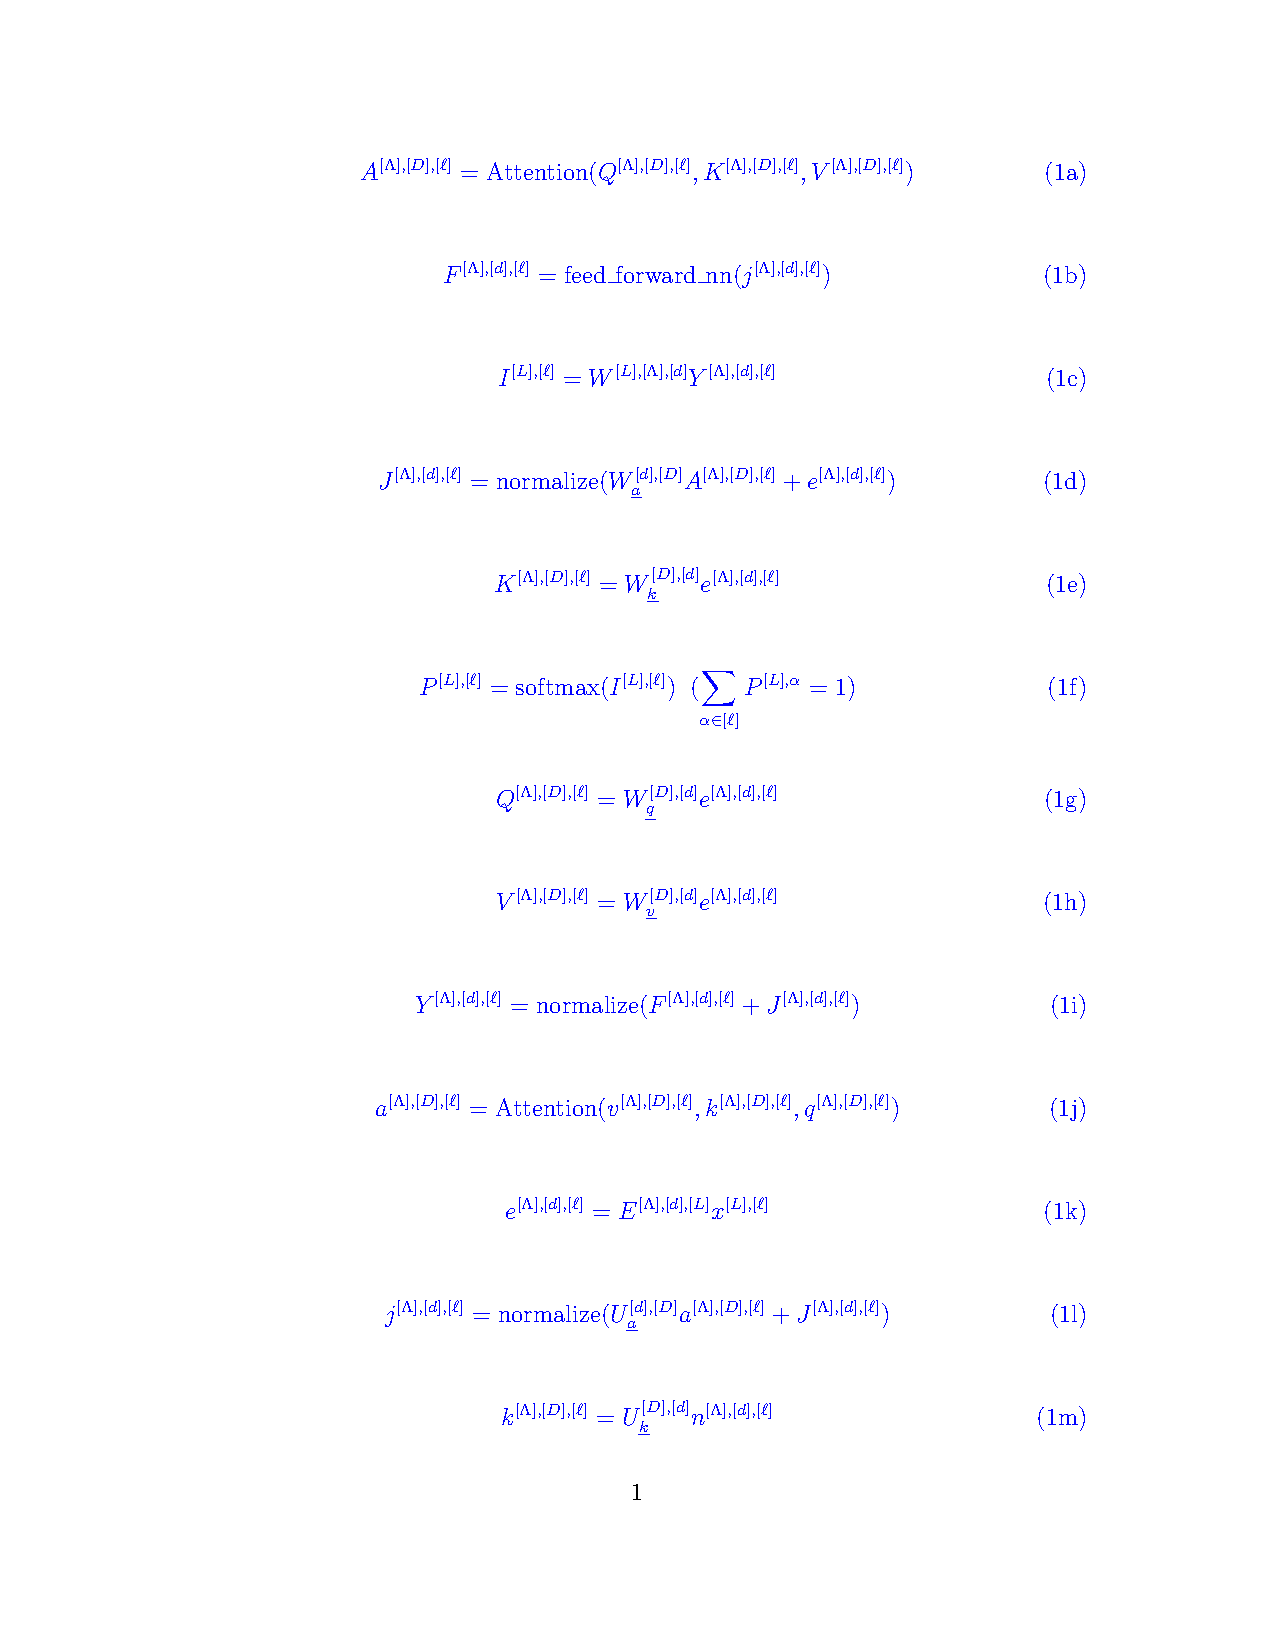
\includegraphics[width=2in]{decoder.jpg}
\end{minipage}%blank lines between minispaces breaks this
\begin{minipage}{.5\linewidth}
$$\xymatrix{
&&&*+[F*:SpringGreen]{\underline{G}^{[L],[\ell]}}
\\
&&&*+[F*:Orchid]{\underline{I}^{[L],[\ell]}}\ar[u]
\\
&&&*+[F*:yellow]{\underline{Y}^{[D], [\ell]}}\ar[u]
\\
&&*+[F*:SkyBlue]{\underline{F}^{[D], [\ell]}}\ar[ur]&
\\
&&&*+[F*:yellow]{\underline{j}^{[D], [\ell]}}\ar[ul]\ar[uu]
\\
&*+[F*:Dandelion]{\underline{o}^{[D],[\ell]}}\ar[urr]&&
\\
*+[F*:Dandelion]{\underline{q}^{[D], [\ell]}}\ar[ur]&*+[F*:Dandelion]{\underline{k}^{[D], [\ell]}}\ar[u]&*+[F*:Dandelion]{\underline{v}^{[D], [\ell]}}\ar[ul]&*+[F*:yellow]{\underline{a}^{[D], [\ell]}}\ar[uu]\ar[l]
\\
&*+[F*:Dandelion]{\underline{O}^{[D],[\ell]}}\ar[urr]&&
\\
*+[F*:Dandelion]{\underline{Q}^{[D], [\ell]}}\ar[ur]&*+[F*:Dandelion]{\underline{K}^{[D], [\ell]}}\ar[u]&*+[F*:Dandelion]{\underline{V}^{[D], [\ell]}}\ar[ul]&
\\
&&&*+[F*:gray]{\underline{p}^{[D],[\ell]}}\ar[ull]\ar[ulll]\ar[ul]\ar[uuu]
\\
&&&*+[F*:Lavender]{\underline{R}^{[L],[\ell]}}\ar[u]
}$$
\end{minipage}
\caption{Decoder.}
\label{fig-texnn-for-decoder}
\end{figure}

\begin{subequations}

\begin{equation}\color{blue}
F^{[D], [\ell]} = {\rm feed\_forward\_nn}(j^{[D], [\ell]})
\label{eq-F-fun-decoder}
\end{equation}

\begin{equation}\color{blue}
G^{[L],[\ell]} = I^{[L],[\ell]}
\label{eq-G-fun-decoder}
\end{equation}

\begin{equation}\color{blue}
I^{[L],[\ell]} = W^{[L], [D]}Y^{[D], [\ell]}
\label{eq-I-fun-decoder}
\end{equation}

\begin{equation}\color{blue}
K^{[D], [\ell]} = p^{[D],[\ell]}
\label{eq-K-fun-decoder}
\end{equation}

\begin{equation}\color{blue}
O^{[D],[\ell]} = {\rm multi\_head\_attention}(Q^{[D], [\ell]},K^{[D], [\ell]},V^{[D], [\ell]})
\label{eq-O-fun-decoder}
\end{equation}

\begin{equation}\color{blue}
Q^{[D], [\ell]} = p^{[D],[\ell]}
\label{eq-Q-fun-decoder}
\end{equation}

\begin{equation}\color{blue}
R^{[L],[\ell]} = 
\label{eq-R-fun-decoder}
\end{equation}

\begin{equation}\color{blue}
V^{[D], [\ell]} = p^{[D],[\ell]}
\label{eq-V-fun-decoder}
\end{equation}

\begin{equation}\color{blue}
Y^{[D], [\ell]} = {\rm normalize}(F^{[D], [\ell]} + a^{[D], [\ell]})
\label{eq-Y-fun-decoder}
\end{equation}

\begin{equation}\color{blue}
a^{[D], [\ell]} = {\rm normalize}(O^{[D],[\ell]} + p^{[D],[\ell]})
\label{eq-a-fun-decoder}
\end{equation}

\begin{equation}\color{blue}
j^{[D], [\ell]} = {\rm normalize}(o^{[D],[\ell]} + a^{[D], [\ell]})
\label{eq-j-fun-decoder}
\end{equation}

\begin{equation}\color{blue}
k^{[D], [\ell]} = 
\label{eq-k-fun-decoder}
\end{equation}

\begin{equation}\color{blue}
o^{[D],[\ell]} = {\rm multi\_head\_attention}(q^{[D], [\ell]},k^{[D], [\ell]},v^{[D], [\ell]})
\label{eq-o-fun-decoder}
\end{equation}

\begin{equation}\color{blue}
p^{[D],[\ell]} = R^{[L],[\ell]}
\label{eq-p-fun-decoder}
\end{equation}

\begin{equation}\color{blue}
q^{[D], [\ell]} = 
\label{eq-q-fun-decoder}
\end{equation}

\begin{equation}\color{blue}
v^{[D], [\ell]} = a^{[D], [\ell]}
\label{eq-v-fun-decoder}
\end{equation}

\end{subequations}


\end{document}  
